\documentclass[a4paper,12pt]{scrartcl}
\usepackage[utf8]{inputenc}
\usepackage[ngerman]{babel}
\usepackage[T1]{fontenc}
\usepackage{amsmath}
\usepackage{stmaryrd}
\usepackage{wasysym}
\usepackage{lmodern}
\usepackage{graphicx}
\usepackage{paralist}
\usepackage{upgreek}
\usepackage{subfigure}
\usepackage{tipa}
\usepackage{amssymb}
\usepackage{gensymb}
\usepackage{dsfont}
\usepackage{mathtools}
\usepackage{ stmaryrd }
\usepackage{fancyhdr}

%\title{Abgabe 1}
%\author{Rafael Heid, Julian Deinert, Sabrina Buczko Gruppe\\ 6 und 7}
%\date{Abgabe am 24.10.16}

\gdef\blatt{FGI-2 Aufgabenblatt 05}

\title{\blatt}
\date{Gruppe 06}
\author{Sabrina Buczko 6663234, Julian Deinert 6535880, Rafael Heid 6704828}


\pagestyle{fancy}
\fancyhf{}
\fancyhead[L]{\blatt}
\fancyhead[R]{Buczko, Deinert, Heid}
\fancyfoot[C]{\thepage}

\begin{document}
\maketitle
\newpage
\setcounter{section}{4}
\section{}
\setcounter{subsection}{2}
\subsection{}
\subsubsection{}
$f = \mathbf{AF}(\neg(orbit \Rightarrow away)))\land \neg \mathbf{AG}(\mathbf{E}(orbit\mathbf{U}warp))$\\
$\Leftrightarrow \mathbf{AF}(\neg(\neg orbit \lor away)) \land \neg\neg \mathbf{EF}(\neg\mathbf{E}(orbit\mathbf{U}warp))$\\
$\Leftrightarrow \neg\mathbf{EG}(\neg orbit \lor away) \land \mathbf{E}(True\mathbf{U}(\neg \mathbf{E}(orbit\mathbf{U}warp)))$\\\\
$g_1 = \mathbf{AGEF}(warp)$\\
$\Leftrightarrow \neg\mathbf{EF}(\neg\mathbf{EF}(warp))$\\
$\Leftrightarrow \neg\mathbf{E}(True\mathbf{U}(\neg\mathbf{E}(True\mathbf{U}warp)))$\\\\
$g_2 = \mathbf{EFAG}(warp)$\\
$\Leftrightarrow \mathbf{E}(True\mathbf{U}(\neg\mathbf{EF}(\neg warp))) $\\
$\Leftrightarrow \mathbf{E}(True\mathbf{U}(\neg\mathbf{E}(True\mathbf{U}\neg warp))) $
\subsubsection{}
Für f: Für alle Pfade vom aktuellen Zustand gilt irgendwann in der Zukunft, dass orbit away nicht impliziert und auf mind. einem Pfad vom aktuellen Zustand aus nicht für immer gilt, dass es einen Pfad ab dem aktuellen Zustand gibt auf dem orbit Until warp gilt.\\
Für $g_1$: Für alle Pfade vom aktuellen Zustand aus gilt immer dass es einen Pfad gibt für den irgendwann in der Zukunft warp gilt.\\
Für $g_2$: Es gibt einen Pfad vom aktuellen Zustand aus für den irgendwann in der Zukunft für alle Pfade immer warp gilt.

\subsubsection{}
$Sat(f)= \{s_1, s_0\}$\\
$Sat(g_1)= S$\\
$Sat(g_2)= \emptyset$
\subsubsection{}
Für $g_1$:\\
$g_1$ gilt auf $M$, da aus der Konstruktion von $M$ ersichtlich ist, 
dass es immer einen Pfad gibt, nach dem irgendwann $warp$ gilt.\\\\
Für $g_2$:\\
Für $g_2$ lässt sich sagen, dass $g_2$ nicht immer auf $M$ gilt, da immer ein Pfad exisitert, nachdem irgendwann in der Zukunft $\neg warp$ gilt und somit nicht für alle Pfade irgendwann $warp$ gilt.

\subsection{}
\subsubsection{}
Die Transitionssysteme der drei Roboter sehen wie folgt aus:\\
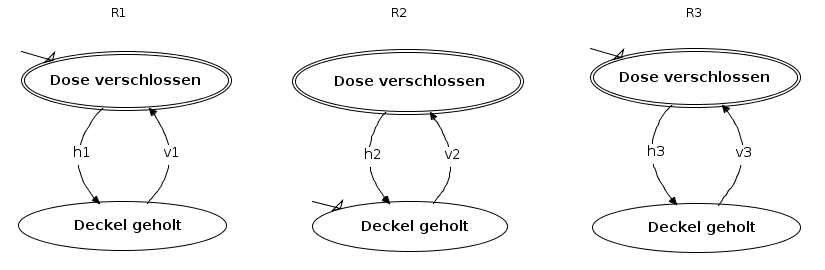
\includegraphics[scale=0.5]{roboter_trans.png}\\
Wobei $h_i$ und $v_i$ jeweils die, den Robotern aufgetragenen Aufgaben widerspiegeln.
\subsubsection{}
Folgendes Produkttransitionssystem entsteht aus den Transitionssystemen der drei Roboter:\\
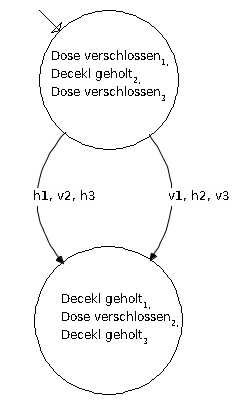
\includegraphics[scale=0.5]{roboter_prod.png}\\
Dabei haben wir eine Synchronisationsrelation $Sync = \{(h1, v2, h3), (v1, h2, v3)\}$
\subsubsection{}
geg.: $\phi = G\lnot((v_1 \land v_2) \lor (v_3 \land v_2))$\\
Umformung zu $\lnot\phi$:\\
\begin{tabular}{ll}
$\lnot\phi$&$=\lnot G\lnot((v_1 \land v_2) \lor (v_3 \land v_2))$\\
&$=F(\lnot\lnot((v_1 \land v_2) \lor (v_3 \land v_2))$\\
&$=F((v_1 \land v_2) \lor (v_3 \land v_2))$
\end{tabular}\\
Folgender Büchi-Automat akzeptiert dieselbe Sprache:\\
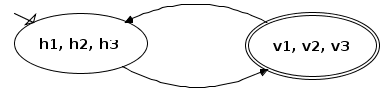
\includegraphics[scale=0.5]{roboter_buechi.png}
\subsubsection{}

\subsection{}
\subsubsection{}
Die richtigen Antworten sind fett gedruckt.\\\\
Was kann ein Nachrichtenmodell?\\
- \textbf{lokale Rechenschritte ausführen}\\
- empfangene Nachrichten löschen oder ändern\\
- \textbf{Nachrichten an andere versenden}\\
- prüfen ob eine Nachricht korrekt übermittelt wurde\\\\\\
Sei $\phi$ ein Ereignis von $p_i$. Was bezeichnet $LT(\phi)$?\\
\textbf{- den von $\phi$ berechneten Wert.\\}
- die von $\phi$ versandten Nachrichten\\
\\\
Für die Ereignisse $\phi_1 ,\phi_2\in\Phi$ gilt $\phi_1$ vor $\phi_2\Leftarrow LT(\phi_1)=LT(\phi_2)$\\
- Wahr\\
- \textbf{Falsch}\\\\\
Welche Prinzipien sollen durch das Beispiel der Petrinetze erläutert werden?\\
- \textbf{Lokalität}\\
- Erreichbarkeit\\
- Stabiliät\\
- Zeittransfer\\
- \textbf{Nebenläufigkeit}\\
- \textbf{grafische und formaltextuelle Darstellung}\\\\\\
Wie finden Transitionen mit disjunkter Lokalität statt?\\
- abhängig\\
- \textbf{unabhängig}\\
% \end{itemize}
\end{document}
